%! suppress = MissingImport
\usepackage{listings}
\usepackage{svg}


\chapter{Theoretical background}


\section{Protein structure prediction problem}
Protein structure prediction is a key problem in computational biology~\cite{alphafold3}, which involves determining the three-dimensional structure of a protein based on its amino acid sequence.
The spatial structure of a protein directly affects its biological function, and accurate conformation prediction allows understanding protein mechanisms and designing new drugs.
This is a difficult task due to the enormous number of possible conformations and complex interactions between atoms.
This problem becomes particularly important for proteins whose structures could not be determined by experimental methods due to technical difficulties.
The application of predicted structures in personalized medicine and pharmacy represents one of the most promising directions in modern biotechnology.

\subsection{Encoding three-dimensional protein structure}
Amino acids in the polypeptide chain encode the spatial structure of the protein through their sequence and physicochemical properties.
Each amino acid has specific features, such as hydrophobicity, electrical charge, or size, which determine possible interactions and arrangement in space~\cite{protein_folding}.
The arrangement of amino acids in space is encoded in the so-called conformational code, which describes different levels of protein structure organization.

The spatial structure of a protein is described at several hierarchical levels of organization:

\begin{itemize}
    \item Primary structure-linear sequence of amino acids connected by peptide bonds, which contains all information necessary to form the native structure
    \item Secondary structure-local structural motifs formed by hydrogen bonds between peptide groups, such as alpha helices and beta sheets
    \item Tertiary structure-global arrangement of the entire polypeptide chain stabilized by various interactions between amino acids
    \item Quaternary structure-the way multiple polypeptide chains associate into a functional protein complex
\end{itemize}

\subsection{X-ray crystallography}
X-ray crystallography is the fundamental experimental method for determining protein structures~\cite{xray_crystallography}, which involves analyzing the diffraction of X-rays on a protein crystal.
X-rays scatter on the electrons of atoms forming the protein, and the diffraction pattern is recorded and mathematically analyzed.
Based on this, an electron density map is created, the analysis of which requires complex mathematical algorithms and knowledge of crystallography.
Interpretation of electron density maps is a challenge often requiring manual fitting of the protein model by experienced researchers.

The process of protein crystallization is often the most difficult stage, requiring significant financial investments and advanced laboratory infrastructure.

\subsection{Computational methods for protein structure prediction}
Computational methods for protein structure prediction are divided into several main categories, among which homology-based methods use sequence similarity to proteins with known structures.
Ab initio methods attempt to predict structure solely based on sequence and laws of physics~\cite{ab_initio_protein_folding}, while fold recognition methods match the sequence to known structural motifs.
Each of these methods has its limitations and works best under specific conditions, depending on the availability of reference data.
Hybrids of these methods often give better results than single approaches, combining advantages of different prediction techniques.

Traditional computational approaches include molecular dynamics simulations and Monte Carlo methods, which use force fields to describe interactions between atoms.
These calculations are very computationally expensive and often limited to small proteins, but in recent years, machine learning and deep learning methods have achieved significant success in this area.
Advances in computational hardware, particularly in the area of GPU accelerators and specialized tensor processors, have significantly accelerated protein structure calculations.
The development of cloud infrastructure has enabled democratization of access to advanced bioinformatics tools.

A breakthrough in the field was the development of the AlphaFold algorithm by Google DeepMind, which uses neural networks to predict protein structures with accuracy comparable to experimental methods.
AlphaFold2 revolutionized the field by winning the CASP14~\cite{casp} (Critical Assessment of protein Structure Prediction) competition in 2020~\cite{alphafold2}.
Deep learning methods have significantly accelerated the pace of scientific discoveries in structural biology, and the public release of the AlphaFold model has enabled researchers worldwide to use this technology in research and medical projects.
Integration of AlphaFold results with other bioinformatics techniques has opened new possibilities in protein-protein interaction analysis and drug design.
The latest version of the algorithm-AlphaFold 3-achieves protein structure prediction accuracy at the level of 90-95\% for single polypeptide chains, and for protein complexes, the accuracy reaches 80-85\%, which represents significant progress compared to previous versions~\cite{alphafold3}.


\section{AlphaFold algorithm by Google Deepmind}

\subsection{Preliminary information}

\subsection{Algorithm implementation}

\subsection{Program operation overview}

\subsection{Required computational resources}


\section{Computing in a computational cluster}

\subsection{Kubernetes Platform}

Kubernetes is an open-source container orchestration software that automates the deployment, scaling, and management of applications~\cite{kubernetes}.
It is currently the main solution in the area of computational cluster management.
Kubernetes originates from Google's internal project called Borg, which was released as an open-source project in 2014.

The main goal of Kubernetes is to provide a platform for running applications in a distributed environment.
The system enables automatic management of computational resources in a heterogeneous hardware environment, encompassing different processor architectures and dedicated computational accelerators.
Kubernetes eliminates many manual processes related to deploying and scaling containerized applications.
All cluster components are controlled declaratively.

The Kubernetes architecture is based on a master-worker node model.
The main control component (control plane) manages worker nodes, on which actual applications are run in containers.
Each Kubernetes cluster consists of at least one master node and many worker nodes.
This architecture provides high availability and fault tolerance.

The resource model in Kubernetes is declarative.
Pod is the basic deployment unit in Kubernetes, representing one or more containers that share resources and are always run on the same cluster node.
After loading a configuration file in YAML format, Kubernetes will strive to bring the actual state of the cluster to the state declared in the configuration.
An example of a Deployment resource declaration shown in listing~\ref{lst:kube-deployment} contains comments explaining key elements:

\begin{lstlisting}[language=yaml,caption={Example Deployment declaration in Kubernetes},label={lst:kube-deployment}]
apiVersion: apps/v1
# Kubernetes resource type
kind: Deployment 
metadata:
  name: nginx-deployment
  labels:
    app: nginx
spec:
  # Number of replicas (copies) of the pod to run
  replicas: 3
  # Selector specifying which pods belong to the deployment
  selector:
    matchLabels:
      app: nginx
  # Template defining pod specification
  template:
    metadata:
      labels:
        app: nginx
    spec:
      containers:
      # Container definition to run
      - name: nginx
        image: nginx:1.14.2
        ports:
        - containerPort: 80  # Port to listen on in the container
\end{lstlisting}

Kubernetes introduces an abstraction of the infrastructure layer.
This allows applications to be moved between different cloud providers without modifying code.
The platform supports various runtime environments, from local clusters, through private clouds, to major public cloud providers.

Key capabilities of Kubernetes include:
\begin{itemize}
    \item Automatic application recovery in case of failure
    \item Load balancing and network traffic distribution
    \item Automatic horizontal scaling of applications based on load
    \item Configuration and secrets management
    \item Persistent storage management
    \item Batch execution for batch jobs and computation scheduling
\end{itemize}

Kubernetes was designed as an extensible platform.
It allows creating custom controllers and operators tailored to specific needs.
This extensibility is key for the KubeFold project, which uses these mechanisms to orchestrate complex protein conformation prediction tasks.

\subsection{Architecture and components of a Kubernetes cluster}

A Kubernetes cluster consists of two main parts: the control node (Control Plane) and worker nodes.
The control node contains components that manage the entire cluster and store its state.

Key components run on the control node: the API Server, which is the access point to the cluster, the Scheduler responsible for assigning tasks to nodes, and the Controller Manager supervising the cluster state.
The etcd database is responsible for storing the cluster state.

Worker nodes run actual workloads in the form of containers.
Each node runs kubelet, which manages containers, and kube-proxy, which handles network traffic.
Containers are grouped into Pods, which are the basic deployment unit.

Kubernetes defines higher-level abstractions such as Deployment or StatefulSet.
They enable declarative application management.
Service provides a stable access point to a group of Pods.

The cluster uses a plugin system to extend functionality.
This includes storage, network, or monitoring drivers.
Particularly important are Custom Resource Definitions, which allow adding custom resource types.

The Kubernetes architecture ensures high availability, scalability, and fault tolerance.
Components can be duplicated across nodes.
The system automatically responds to failures by restarting and relocating applications.

\subsection{Available resources in the computational cluster}
Kubernetes platform defines basic resource types used to manage applications in a computational cluster.
Each resource type serves a specific role and can be configured by administrators and applications.

\subsubsection{Pod}
Pod is the basic deployment unit in a Kubernetes cluster.
It represents a process executing an application along with its execution context.
A Pod contains one or more containers sharing network space and storage resources.
Listing~\ref{lst:pod-example} shows an example definition of a Pod with an application server and an attached data volume.

\begin{lstlisting}[language=yaml,caption={Example Pod definition},label={lst:pod-example}]
apiVersion: v1
kind: Pod
metadata:
  name: web-server
  labels:
    app: web
spec:
  containers:
  - name: nginx
    image: nginx:latest
    resources:
      limits:
        memory: "128Mi"
        cpu: "500m"
    volumeMounts:
    - name: www-data
      mountPath: /usr/share/nginx/html
  volumes:
  - name: www-data
    persistentVolumeClaim:
      claimName: web-content
\end{lstlisting}

\subsubsection{Job}
Job represents a computational task with a finite execution time.
This resource guarantees successful execution of a specified number of Pods.
In case of a computational node failure, the Job automatically creates a new Pod instance.
Listing~\ref{lst:job-example} shows an example of a Job performing batch file conversion.

\begin{lstlisting}[language=yaml,caption={Example Job definition},label={lst:job-example}]
apiVersion: batch/v1
kind: Job
metadata:
  name: batch-convert
spec:
  template:
    spec:
      containers:
      - name: converter
        image: imagemagick:latest
        command: ["convert"]
        args: ["*.jpg", "-resize", "800x600", "output/"]
      restartPolicy: Never
  backoffLimit: 4
\end{lstlisting}

\subsubsection{PersistentVolume}
PersistentVolume defines a persistent storage volume in the cluster.
It is independent of the Pod lifecycle and stores data that must survive cluster restarts.
Listing~\ref{lst:pv-example} shows the definition of a volume using the NFS file system.

\begin{lstlisting}[language=yaml,caption={Example PersistentVolume definition},label={lst:pv-example}]
apiVersion: v1
kind: PersistentVolume
metadata:
  name: nfs-volume
spec:
  capacity:
    storage: 100Gi
  accessModes:
    - ReadWriteMany
  persistentVolumeReclaimPolicy: Retain
  nfs:
    server: nfs-server.example.com
    path: "/shared"
\end{lstlisting}

\subsubsection{PersistentVolumeClaim}
PersistentVolumeClaim is a request for allocation of storage resources.
It defines requirements regarding the size and access mode for the volume.
Listing~\ref{lst:pvc-example} shows an example request for creating a 10GB volume.

\begin{lstlisting}[language=yaml,caption={Example PersistentVolumeClaim definition},label={lst:pvc-example}]
apiVersion: v1
kind: PersistentVolumeClaim
metadata:
  name: web-content
spec:
  accessModes:
    - ReadWriteMany
  resources:
    requests:
      storage: 10Gi
  storageClassName: standard
\end{lstlisting}

\subsubsection{StorageClass}
StorageClass describes a storage class available in the cluster.
It defines the provider and configuration parameters for volumes.
Listing~\ref{lst:sc-example} shows the definition of a standard storage class for SSD disks.

\begin{lstlisting}[language=yaml,caption={Example StorageClass definition},label={lst:sc-example}]
apiVersion: storage.k8s.io/v1
kind: StorageClass
metadata:
  name: fast-storage
provisioner: kubernetes.io/aws-ebs
parameters:
  type: gp3
  iopsPerGB: "5000"
  encrypted: "true"
reclaimPolicy: Delete
allowVolumeExpansion: true
\end{lstlisting}

\subsection{Volume allocation mechanism}
Kubernetes uses a complex mechanism for dynamic allocation of storage resources.
When an application creates a PersistentVolumeClaim, the system checks the storage class (StorageClass) declared in it.
Based on this, it activates the appropriate driver that creates a physical volume in the infrastructure.
The newly created PersistentVolume is then automatically linked to the claim.
Thanks to this mechanism, a cluster administrator can define different storage classes, and users can use them without knowing the technical details of the infrastructure.
The system guarantees that the volume will exist as long as the claim associated with it exists.
After deleting a PersistentVolumeClaim, the fate of the volume depends on the defined reclaim policy - it can be automatically deleted or preserved for reuse.

\subsection{Kubernetes clusters in the cloud}

Kubernetes clusters in a cloud environment represent a natural evolution of computational platforms.
The cloud offers dynamic resource allocation and integration with services such as data stores or monitoring systems.
Geographic distribution ensures high availability, and automatic backup mechanisms protect against data loss.
Advanced access control systems guarantee the security of data and applications.

Public cloud providers offer managed Kubernetes services that automate most administrative tasks.
This includes cluster creation and configuration, component updates, and infrastructure state monitoring.
Thanks to this, teams can focus on application development instead of infrastructure maintenance.

\subsection{Managed Kubernetes service in Amazon Web Services}

Amazon Elastic Kubernetes Service (EKS) is a comprehensive solution for running Kubernetes clusters in the AWS cloud.
The service automatically manages control node updates, certificates, and network configuration.
Integration with AWS services simplifies creating solutions using data stores or notification systems.

In the context of the KubeFold project, access to instances equipped with graphics cards and integration with the FSx for Lustre file system are of key importance.
EKS enables automatic scaling of the node group depending on demand, which translates into cost optimization.

Using Kubernetes clusters in the cloud brings significant benefits for computational projects.
Elimination of costs for maintaining own infrastructure and access to specialized hardware without the need to purchase allow for flexible budget management.
The billing model based on actual resource consumption works particularly well in the case of computations with varying intensity, such as protein conformation prediction.
Automatic recovery mechanisms after failure and global availability ensure reliability and high-quality services.
This combination of features makes cloud Kubernetes clusters an optimal environment for modern scientific applications.

\subsection{Lustre volumes}

Lustre is a distributed file system, created by Cluster File Systems in 2003.
This system was designed for high-performance computing clusters.
Currently, the development of Lustre is managed by the OpenSFS (Open Scalable File Systems) organization.

The Lustre file system consists of several main components:
\begin{itemize}
    \item Metadata servers (MDS) - store information about the file system structure, directories, and permissions
    \item Object storage servers (OSS) - responsible for storing actual data and handling input/output operations
    \item Clients - nodes that mount the file system and use it
    \item Metadata target devices (MDT) - store metadata on block devices
    \item Object storage targets (OST) - store file data on block devices
\end{itemize}

The Lustre architecture is based on the separation of metadata from actual data.
Metadata servers deal exclusively with operations on directory structure and permissions.
Object servers handle operations on the file data itself.
Such separation allows for optimization of both types of operations independently.

Lustre ensures very high performance through parallel input/output operations.
The system enables simultaneous access to the same files from multiple cluster nodes.
A single Lustre file system can serve tens of thousands of clients simultaneously.
The system's throughput scales linearly with the addition of more object servers.

Main features of the Lustre file system:
\begin{itemize}
    \item High scalability - ability to handle petabytes of data and thousands of nodes
    \item High throughput - ability to achieve throughput in the terabit per second range
    \item Cache coherence - guarantee of data consistency between all clients
    \item Fault tolerance - ability to work despite failure of individual components
    \item Support for multiple access protocols - POSIX, MPI-IO, HDFS
\end{itemize}

In the KubeFold project, Lustre is a key component for storing protein databases.
Its architecture ensures high throughput and low latency when accessing data.
The system allows simultaneous access to files from multiple cluster nodes performing calculations.
This makes it possible to parallel process data by multiple instances of the AlphaFold algorithm.

Lustre is widely used in computing centers around the world.
It is used in supercomputers from the TOP500 list.
The system works particularly well in scientific computing, where processing huge datasets is required.
Examples of applications include physical simulations, climate modeling, and genomic calculations.

\subsection{Amazon S3 object storage}

Amazon Simple Storage Service (S3) is a cloud object storage service.
It provides virtually unlimited disk space with guaranteed availability of 99.999999999\%.
It is an industry standard for cloud data storage.

The basic organizational unit in S3 are buckets.
Each bucket has a globally unique name and can store any number of objects.
Objects are identified by keys, which can contain slash characters to create a hierarchical structure.

S3 has become the standard for data storage in cloud applications.
Most modern cloud solutions provide integration with this system.
Tool providers often implement S3 support as the first choice for integrations with data stores.

The service provides a REST API interface and libraries for many programming languages.
Authentication uses digital signatures or temporary credentials.
Access control is based on IAM policies and ACL lists.
These standard mechanisms are widely used in the cloud ecosystem.

S3 provides full integration with other AWS services.
It is commonly used as storage for backups, a place to store artifacts, or the target location for computation results.
Its reliability and scalability make it the primary choice for applications requiring persistent data storage.

\subsection{AWS End User Messaging Service}

AWS End User Messaging is a service that enables sending SMS messages to end users.
It uses the Amazon Simple Notification Service (SNS) infrastructure to deliver messages.

The service offers the following capabilities:
\begin{itemize}
    \item sending individual SMS messages
    \item sending group messages
    \item monitoring delivery status
    \item managing sending limits
    \item automatic shortening of long messages
\end{itemize}

The system handles two types of SMS messages:
\begin{itemize}
    \item Promotional - optimized for cost
    \item Transactional - optimized for delivery reliability
\end{itemize}

The service provides global reach through cooperation with multiple mobile operators.
Messages can be sent to over 200 countries and territories.
SNS automatically selects the best route for message delivery.

The service billing is based on the number of messages sent.
The price depends on the target country and the chosen message type.
The system offers cost control mechanisms through setting monthly spending limits.

Integration with the service is done through the REST API interface or SDK sets available for popular programming languages.
The service also provides detailed event logs and metrics available in Amazon CloudWatch.

The KubeFold platform uses AWS End User Messaging to notify researchers about the completion of protein structure calculations by the AlphaFold algorithm.
The system sends SMS messages containing information about task status and links to results in S3 storage.


\section{Cluster operator concept}

A Kubernetes operator is a program that extends cluster capabilities with automatic management of complex applications.
An operator automates tasks that would normally require manual intervention from a system administrator.

Custom Resource Definitions (CRDs) are the fundamental building blocks of an operator.
These resources define new types of objects that can be managed within a Kubernetes cluster.
The operator continuously monitors the state of these resources and performs necessary actions to keep the system running as expected.

The operator automates typical administrative tasks such as:
\begin{itemize}
    \item Installing and updating applications
    \item Creating and restoring backups
    \item Detecting and fixing failures
    \item Modifying application settings
\end{itemize}

Operators are particularly effective at managing stateful applications like databases and messaging systems.
In such cases, the operator automatically performs complex operations that typically require specialized knowledge.

An operator consists of two main parts: custom resource definitions and a management program.
The management program continuously compares the current system state with the desired state and implements necessary changes.

\subsection{Cluster operator architecture}

A Kubernetes operator follows a control loop pattern called the reconciliation loop.
This pattern continuously monitors the cluster state and makes adjustments to maintain the desired configuration.
The operator consists of several key components working together to manage custom resources.

The core components of an operator architecture include:

\begin{itemize}
    \item Custom Resource Definition (CRD) - Defines the schema and validation rules for custom resources
    \item Controller - Implements the business logic and reconciliation loop
    \item Client - Interfaces with the Kubernetes API to read and modify resources
    \item Cache - Maintains an in-memory copy of watched resources for efficiency
    \item Work Queue - Buffers reconciliation requests to handle them sequentially
\end{itemize}

The reconciliation loop follows these main steps:
\begin{enumerate}
    \item Watch for changes to custom resources and related Kubernetes objects
    \item Compare current state with desired state specified in the custom resource
    \item Calculate what changes are needed to reach desired state
    \item Apply the necessary changes through the Kubernetes API
    \item Update status of the custom resource
\end{enumerate}

Figure \ref{fig:kubernetes-operator-flow} illustrates the typical interaction flow between components in a Kubernetes operator:

\begin{figure}[htbp]
    \centering
    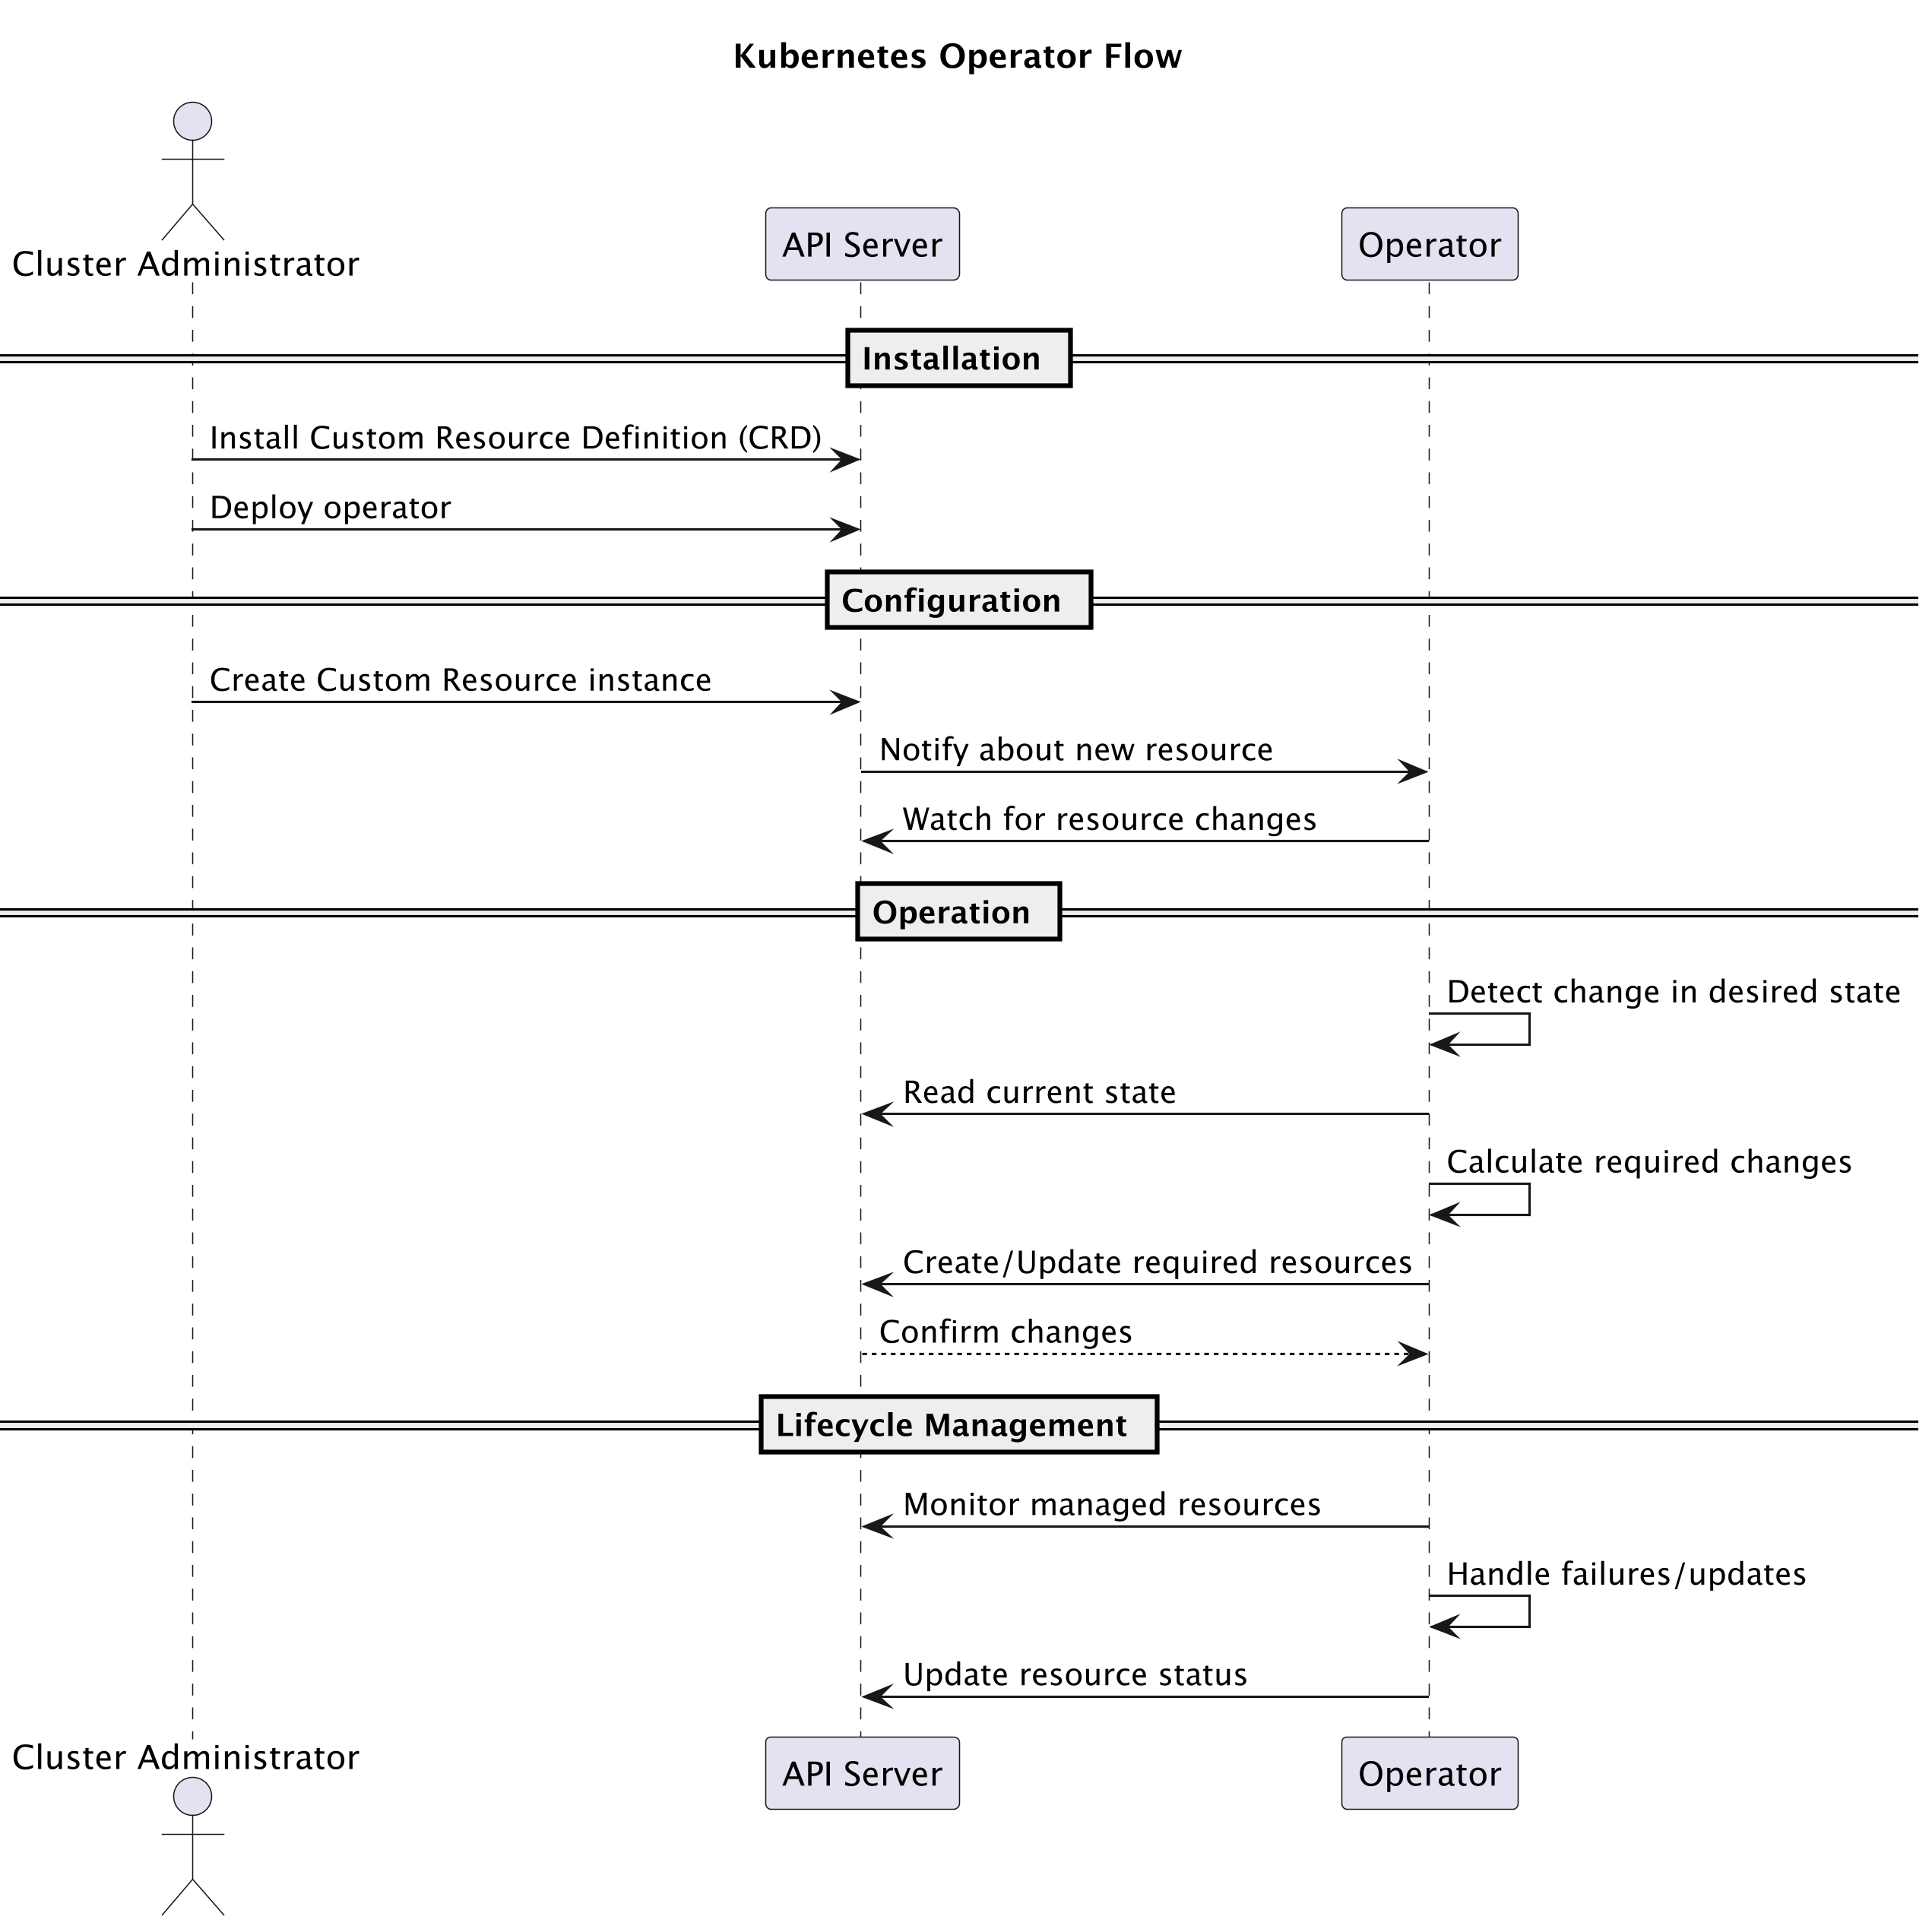
\includegraphics[width=\textwidth]{images/kubernetes_operator_flow.png}
    \caption{Kubernetes Operator Sequence Diagram demonstrating a reconciliation loop}
    \label{fig:kubernetes-operator-flow}
\end{figure}

The operator pattern enables domain-specific knowledge to be encoded into software that can automatically manage complex applications.
This automation reduces operational overhead and helps maintain consistency across deployments.

\subsection{Go programming language}

Go was created in 2007 by a Google team consisting of Robert Griesemer, Rob Pike, and Ken Thompson.
Google needed a language that would streamline the creation of large-scale server systems and simplify the software development process in large programming teams.

The first public version of the language was released in 2009.
The language was created with the intention of building scalable server systems that could handle Google's growing infrastructure.
The creators wanted to combine the simplicity of Python with the efficiency of C.

The main features of Go are simple syntax, built-in concurrency support, and efficient compilation.
The language offers static typing and automatic memory management.
The Go standard library provides rich support for network operations and concurrent processing.

Go introduces communication channels and goroutines as basic mechanisms for handling concurrency.
Thanks to them, creating parallel programs is much simpler than in other languages.
This is particularly useful in distributed systems.

The Go ecosystem provides tools for automatic code formatting, documentation generation, and dependency management.
Go modules enable versioning and easy code sharing.
The \textit{go mod} tool automatically manages project dependencies.

Go is a popular choice for creating DevOps tools and cloud systems.
Kubernetes and Docker were written in Go. This language works well in projects requiring high performance and reliability.